\section{Introduction}

\begin{frame}[c]{Expression du besoin}
	
	\begin{figure}
		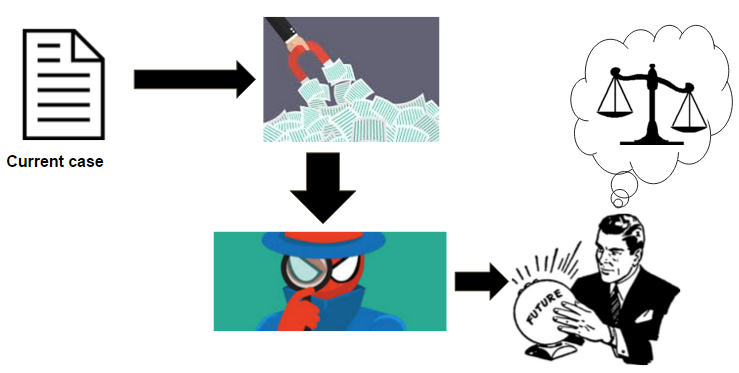
\includegraphics[width=0.7\textwidth]{lawyerwork.png}
		\caption{Les juristes analysent les décisions}
	\end{figure}
	
	\begin{block}{Pourquoi?}
		\begin{itemize}
			\item comprendre et comparer l'application de la loi (contentieux, ville, ...)
			\item estimer le risque judiciaire
			\item ... %anticiper les affaires futures
		\end{itemize}
	\end{block}
\end{frame}

\begin{frame}[c]{Motivation: grand volume de décisions}
	\textbf{Plus de 4 millions de décisions prononcées / an}
	\begin{table}[!htb]
		\scriptsize
		\begin{center}
			\begin{tabular}{|l|l|l|l|l|l|}
				\hline
				\textbf{Justice}	& \textbf{2013}  & \textbf{2014}  & \textbf{2015}  & \textbf{2016}  & \textbf{2017}  \\ \hline
				civile   & 2 761 554 & 2 618 374 & 2 674 878 & 2 630 085 & 2 609 394 \\ \hline
				pénale   & 1 303 469 & 1 203 339 & 1 206 477 & 1 200 575 & 1 180 949 \\ \hline
				administrative & 221 882 & 230 477 & 228 876 & 231 909 & 242 882 \\ \hline
			\end{tabular}
			
			\textit{\tiny{\textbf{Source}: \url{http://www.justice.gouv.fr/statistiques-10054/chiffres-cles-de-la-justice-10303/}}}  
		\end{center}
		\caption{Nombre de décisions prononcées en France par an de 2013 à 2017.}\label{tab:intro:nbdecisionstats}
	\end{table}
\end{frame}

\begin{frame}[t]{Motivation: recherches et analyses sémantiques difficiles}
	
	Moteurs de recherche juridique à mots-clés 
	
	Aucune analyse synthétique des décisions 
	
	%\begin{figure}
	\fbox{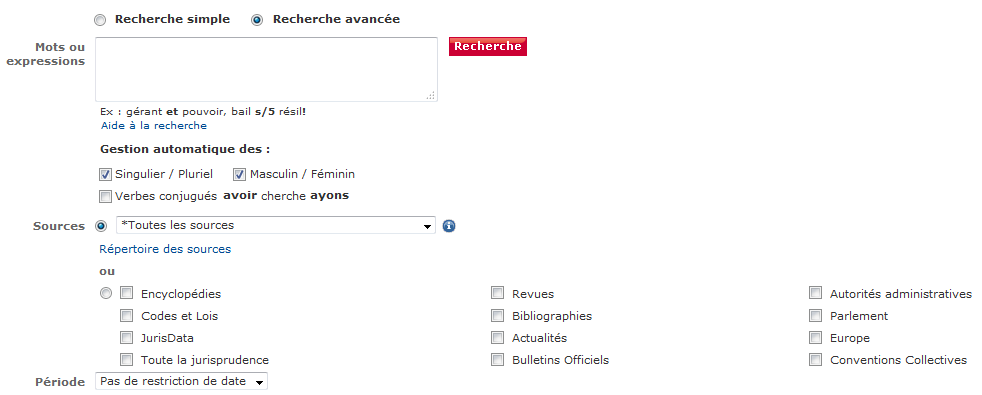
\includegraphics[width=0.9\paperwidth]{jurica.png}}
	
	\textit{\tiny{Source: \url{LexisNexis.com}}} 
	%\caption{Formulaire de recherche}
	%\end{figure}
\end{frame}

\begin{frame}[c]{État de l'art : analyse automatique de décisions judiciaires}
	\scriptsize
	\begin{itemize}
		\item Extraction d'information dans les décisions
		\begin{itemize}  \scriptsize
			\item entités juridiques \cite{Waltl2016lexia, andrew2018legalNerAndRelation}
			\item faits \cite{wyner2010extractlegalelts, wyner2010casefactors, Shulayeva2017recognfactprincip}
			\item définitions de concept juridiques \cite{Waltl2016lexia,waltl2017legaliegerman}
			\item arguments \cite{moens2007NBvsMaxent4arguments}
		\end{itemize}
		\item Classification de décisions
		\begin{itemize} \scriptsize
			\item Prédiction des décisions de justice \cite{Ashley2009classifCases, Aletras2016predictDecisionECHR}
			\item identification de la formation et la période \cite{Sulea2017predictareadecision,sulea2017legalEnsSVM}
			\item identifier la sentence prononcée (Chine) \cite{ma2018wmdchinesecase}
		\end{itemize}
		\item Similarité entre décisions 
		\begin{itemize}  \scriptsize
			\item décisions qui citent les mêmes lois et précédents \cite{nair2018judgsimassorule}
			\item recherche d'affaires antérieures pertinentes  \cite{thenmozhi2017legalprecedretriev}
			\item identifier la sentence prononcée (Chine) \cite{ma2018wmdchinesecase}
			\item similarité basée sur la question discutée et les faits sous-jacents (Inde) \cite{kumar2011judgmentsimilarity}
			\item regroupement non-supervisé \cite{raghuveer2012legalclusteringLDA}
		\end{itemize}
	\end{itemize}
\end{frame}

\begin{frame}[c]{Objectif : automatiser des tâches d'analyse de décisions}
%	\only<1>{
		\begin{figure}[!htb]
		% pipeline-cassandra.pdf
		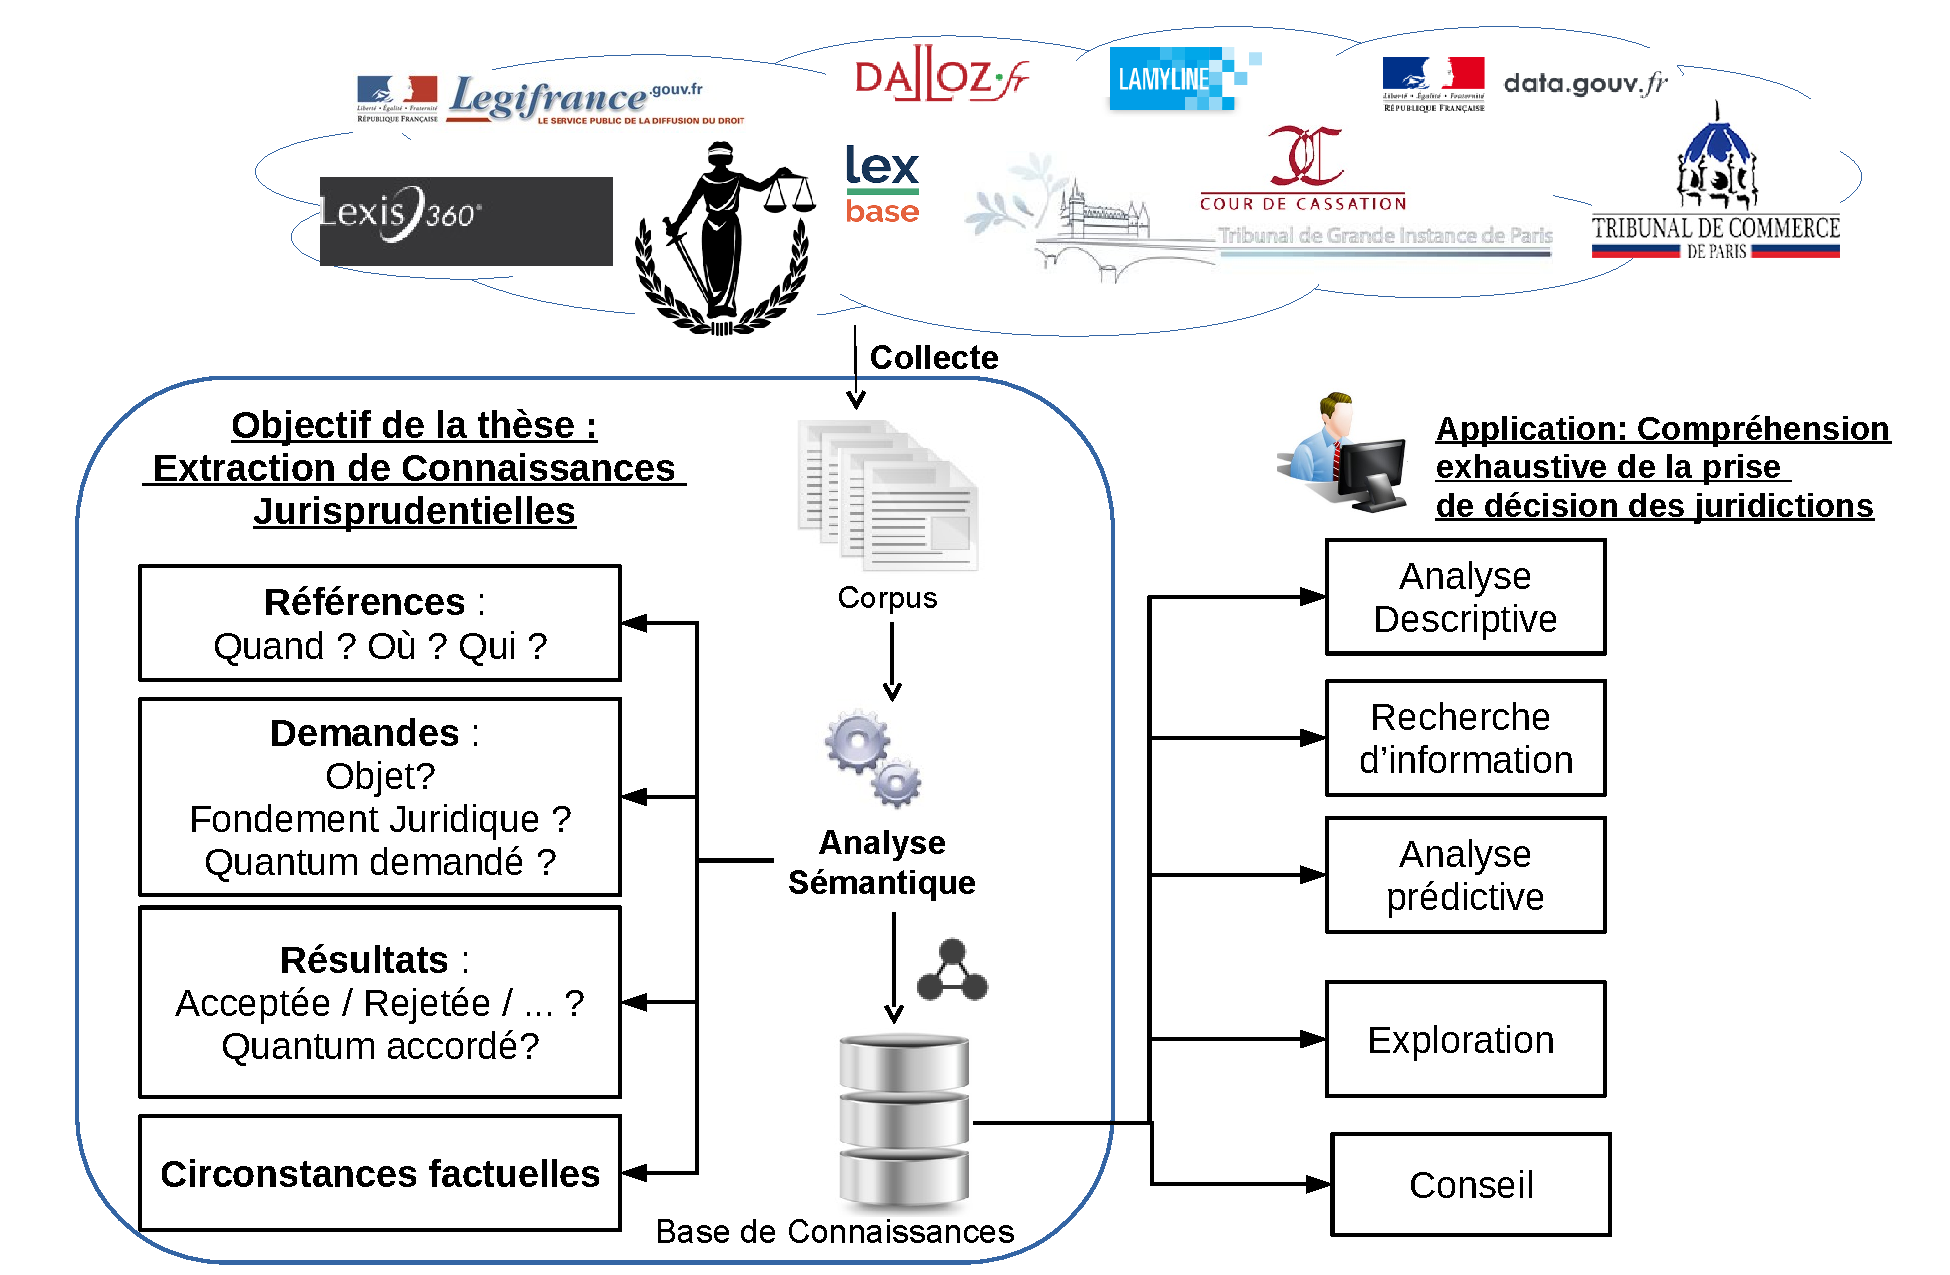
\includegraphics[width=\textwidth]{Objectif_these.pdf}
		\caption{Objectifs et exemples d'application de la thèse.} \label{fig:intro:objectif-these}
	\end{figure}
%}

%	\only<2>{\begin{figure}[!htb]
%		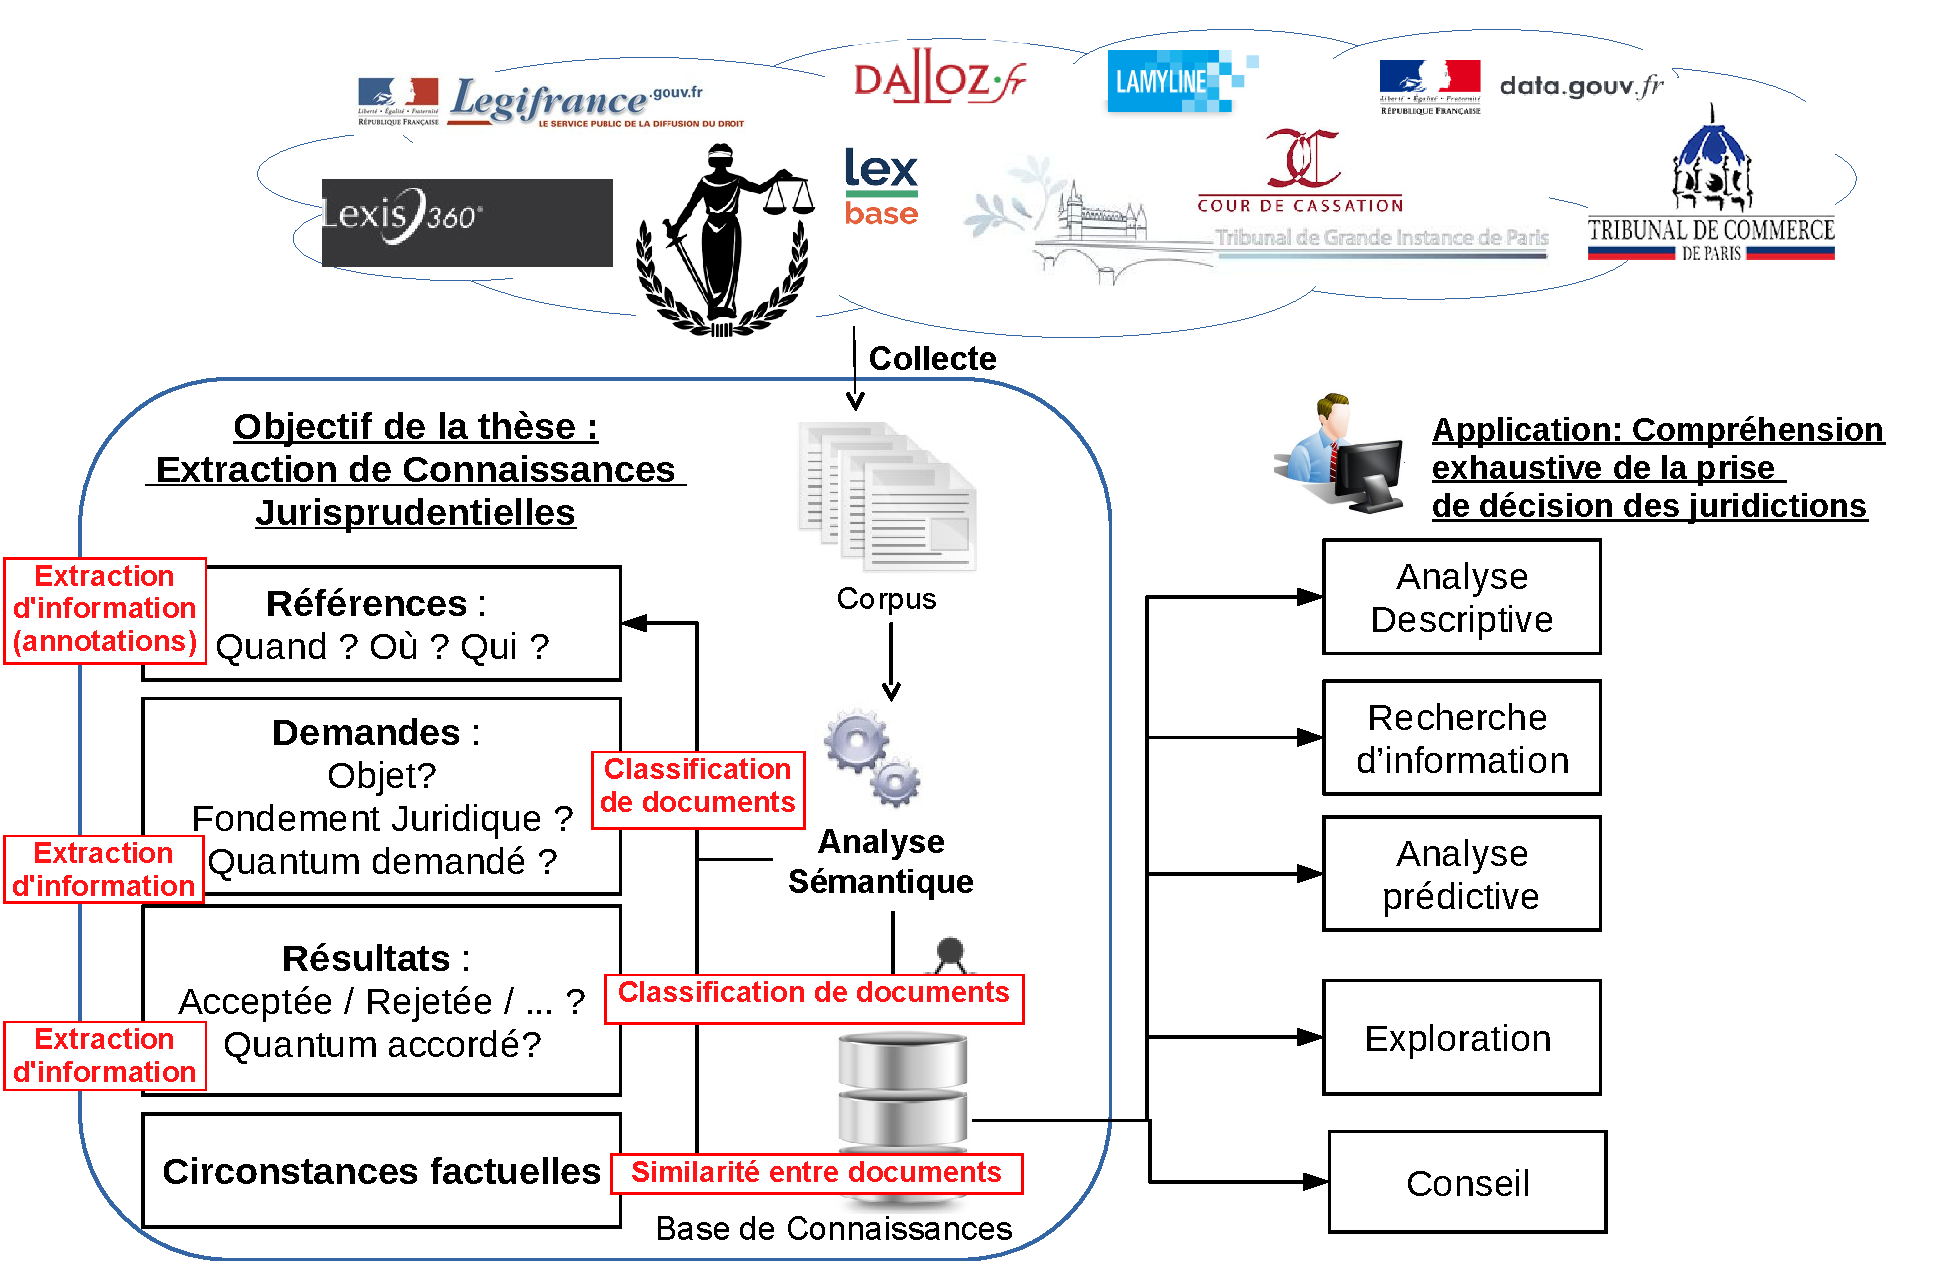
\includegraphics[width=\textwidth]{Objectif_these-problemes2.pdf}
%		\caption{Problèmes correspondants en analyse de données textuelles.} \label{fig:intro:objectif-these-problemes}
%	\end{figure}}
\end{frame}

\begin{frame}[c]{Problème : annotation de sections, métadonnées, normes}
    \tiny
	\lstset{language=XMl}
	\begin{columns}
		\begin{column}{.50\linewidth}
        \lstinputlisting{contents/CALYO1406777.xml}
        \end{column}
		\begin{column}{.50\linewidth}
		\lstinputlisting{contents/CALYO1406777-2.xml}
	    \end{column}
	\end{columns}
\end{frame}

\begin{frame}[c]{Problème : extraction des demandes}
	Cibles : sens du résultat, montant demandé, montant accordé
\begin{exampleblock}{Expression de demande et resultat}
%danais/CASAI1401082.xml
\scriptsize
Jennifer M. et Catherine M. ... demandent à la Cour de :

- \textcolor{orange}{infirmer le dit jugement} en \textcolor{blue}{toutes ses dispositions} ; 
...

Statuant à nouveau ...

- les condamner au paiement d' une somme de  \textbf{3 000,00 € pour procédure abusive} et
aux entiers dépens ; ...

La cour ...  

CONFIRME \textcolor{orange}{le jugement entrepris} en \textcolor{blue}{toutes ses dispositions}.

\end{exampleblock}

\scriptsize{\textit{Légende:  \textcolor{orange}{référence au jugement antérieur},  \textcolor{blue}{agrégation}}}


\begin{table} 
\centering 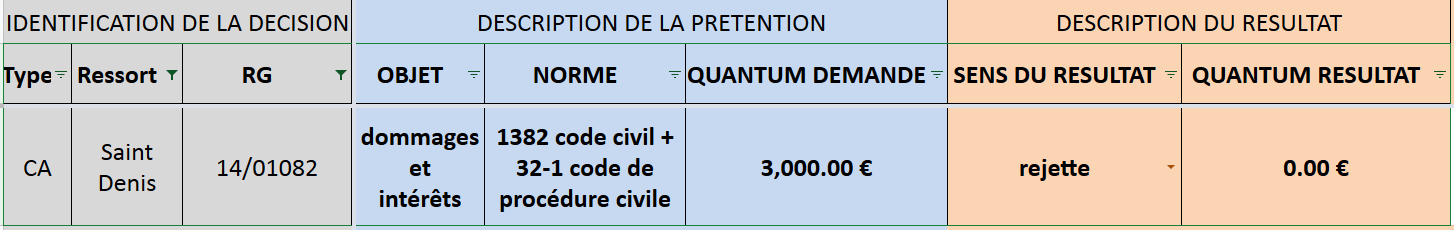
\includegraphics[width=\textwidth]{tab-danais.png}
\caption{\scriptsize Informations à extraire (dommages-intérêts pour procédure abusive)}
\end{table}
\end{frame}

\begin{frame}[c]{Problème : découverte des circonstances factuelles}
  Déterminer les situations distinctes où sont formulées les demandes d'une catégorie données.
    \begin{exampleblock}{Categorie : action en responsabilite civile professionnelle contre les avocats}
	\begin{itemize}
    \item cas $a$ (46 documents): il s'agit d'un avocat négligent qui envoie son assignation de manière tardive ; %(champ sémantique: retard/délai/prescription)
    \item cas $b$ (20 documents): il s'agit d'un avocat qui n'a pas donné un conseil opportun, qui n'a pas soulevé le bon argument;
    \item cas $c$ (18 documents): un avocat qui n'a pas rédigé un acte valide ou réussi à obtenir un avantage fiscal; % (champ sémantique: rédacteur d'actes)
    \item cas $d$ (3 documents): il s'agit d'un avocat attaqué par son adversaire et non par son propre client.
    \end{itemize}
    \end{exampleblock}
\end{frame}

\begin{frame}[c]{Positionnement en fouille de texte}	
	\begin{figure}[!htb]
		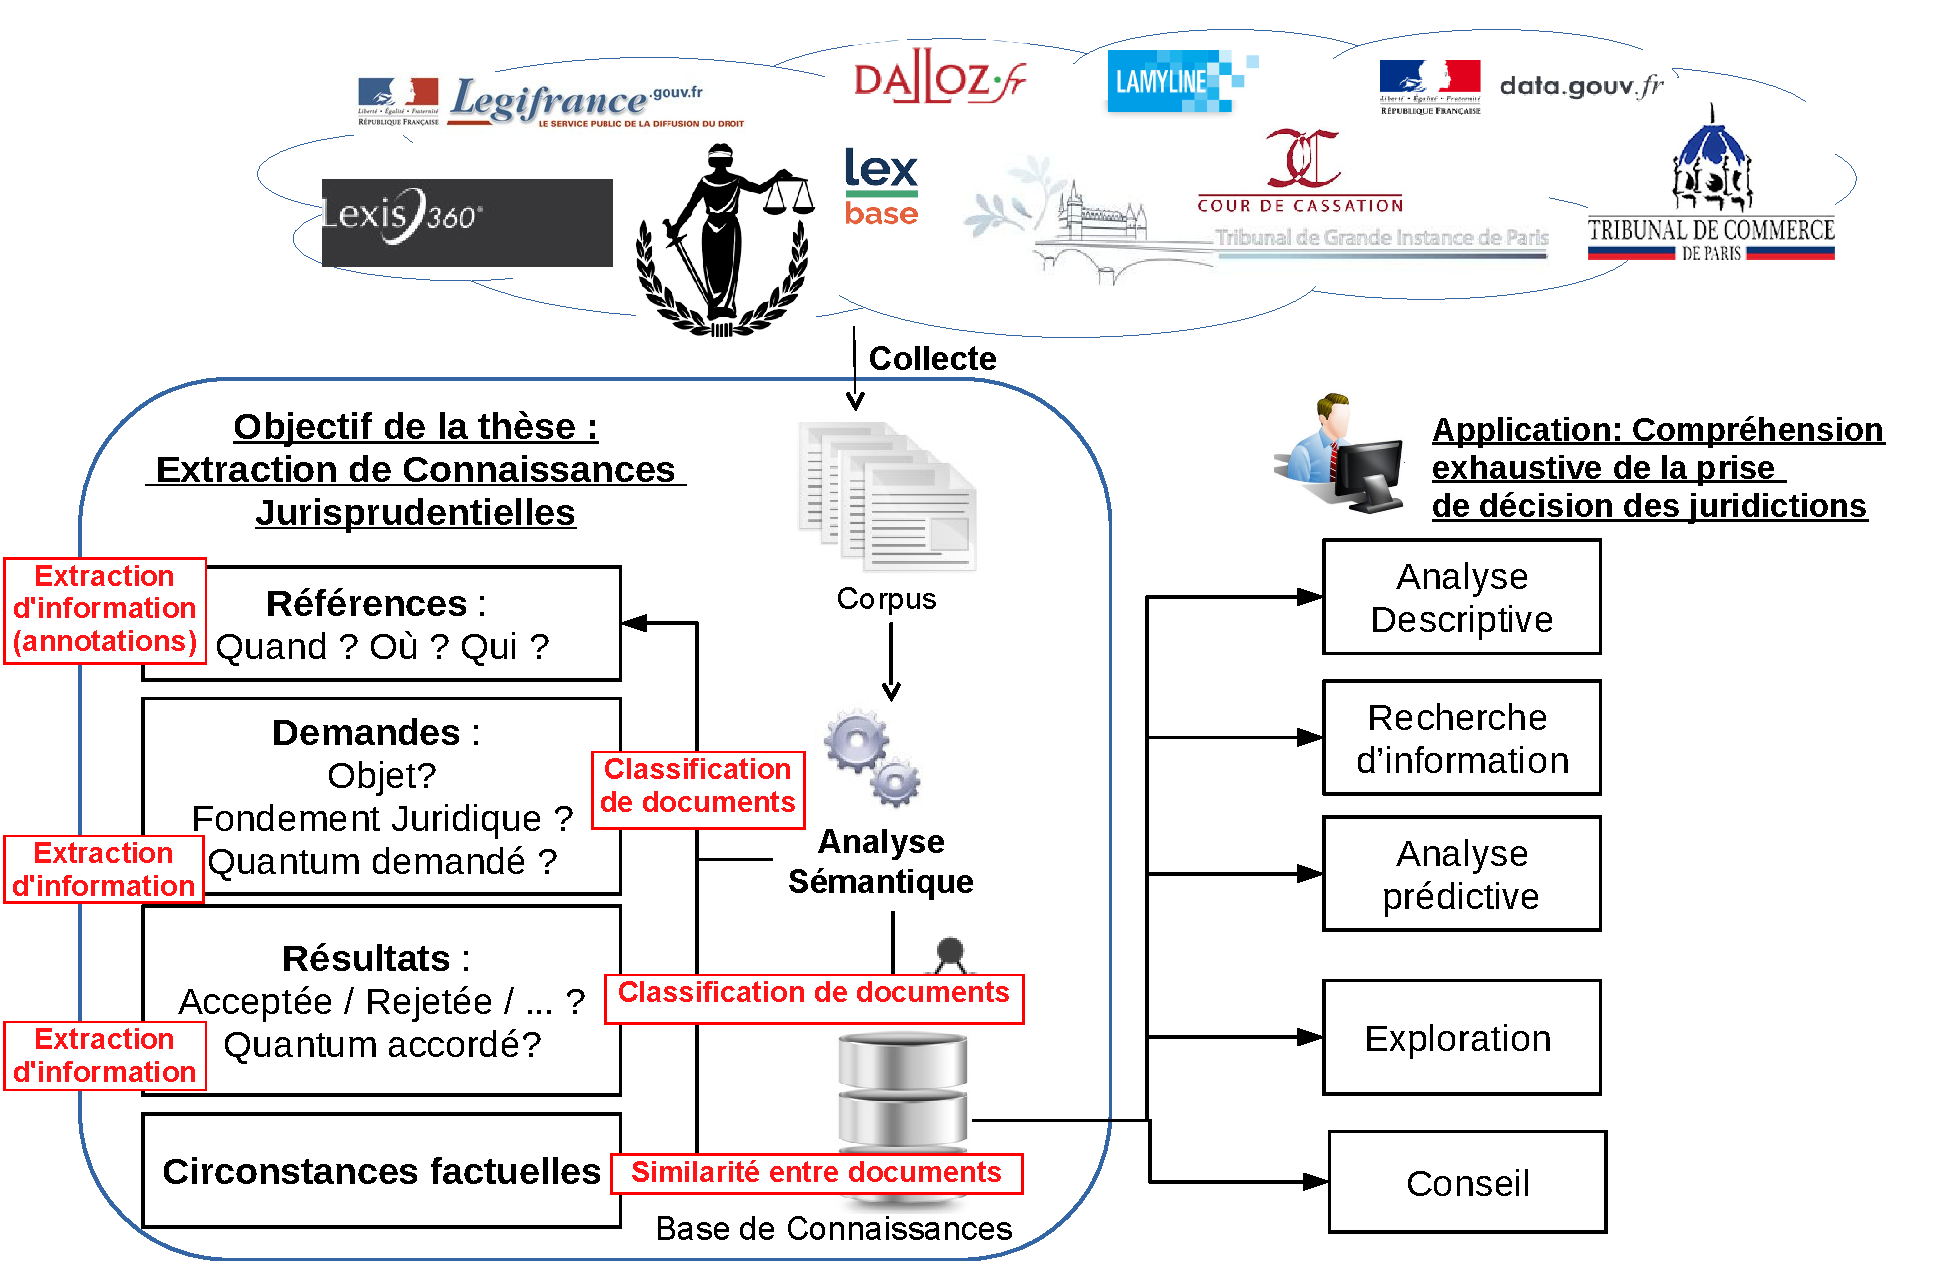
\includegraphics[width=\textwidth]{Objectif_these-problemes2.pdf}
		\caption{Tâches abordées en analyse de données textuelles.} \label{fig:intro:objectif-these-problemes}
	\end{figure}
\end{frame}

\begin{frame}{Difficultés rencontrées par l'automatisation de ces tâches}
	\begin{itemize}
		\item Les décisions sont des textes non-structurés
		\item Le langage juridique est complexe
	\end{itemize}	

	\tiny	
	\begin{columns}
		\begin{column}{.50\linewidth}
			ARRÊT N°
			
			R.G: 11/03924
			
			...
			
			{COUR D'APPEL} DE {NÎMES}
			
			{CHAMBRE CIVILE}
			
			{1ère Chambre A}
			
			ARRÊT DU {20 MARS 2012}
			
			APPELANTE:
			
			{Madame Michéle A.} ...
			
			assistée de la {SELARL VAJOU}, ...
			
			INTIMES:
			
			{Monsieur Martial B} ...
			
			assisté de la {SCP MARION GUIZARD PATRICIA SERVAIS}, ...
			
			COMPOSITION DE LA COUR LORS DU DÉLIBÉRÉ:
			
			{M. Dominique BRUZY, Président}
			
			{M. Serge BERTHET, Conseiller}
			
			...
		\end{column}
		\begin{column}{.50\linewidth}
			FAITS, PROCEDURE, ...
			
			Madame Michèle A. demande:
			
			...
			
			- de condamner Madame JONES-B. à lui payer la somme de {2.500 euros} au titre de l'{article 700 du Code de Procédure Civile}, 
			
			\vspace{0.4cm}
			
			PAR CES MOTIFS, LA COUR:
			
			...
			
			Vu l'{article 809 du Code de Procédure Civile},
			
			...
			
			{Déboute Madame A. de sa demande de provision sur dommages-intérêts.}
			
			...
			
			Vu l'{article 700 du Code de Procédure Civile},
			
			Condamne Madame JONES-B. à verser à Madame A. la somme de {2.500 euros}.
		\end{column}
	\end{columns}
\end{frame}